\documentclass[11pt,a4paper]{article}

\usepackage{amsmath,amssymb,amsthm}
\usepackage{mathtools}
\usepackage{geometry}
\usepackage{booktabs}
\usepackage{array}
\usepackage{tikz}
\usetikzlibrary{matrix,positioning,arrows.meta,calc,decorations.pathreplacing,fit}
\usepackage{hyperref}
\usepackage{xcolor}

\geometry{margin=1in}

\newtheorem{theorem}{Theorem}
\newtheorem{lemma}[theorem]{Lemma}
\newtheorem{property}{Property}
\theoremstyle{definition}
\newtheorem{definition}{Definition}

\title{\textbf{RapidsGEMM}}
\author{Your Name}
\date{}

\begin{document}
\maketitle

\begin{abstract}
\end{abstract}

%=============================================================================
\section{Introduction}
%=============================================================================

%=============================================================================
\section{Background}
%=============================================================================

%=============================================================================
\section{Method}
%=============================================================================

We first define the grouped GEMM operations that arise in MoE training,
then describe our proposed method for implementing them efficiently.

%---------------------------------------------------------------------
\subsection{Problem Definition}
%---------------------------------------------------------------------

A Mixture-of-Experts (MoE) feed-forward network (FFN) routes each token to
its top-$k$ experts~\cite{shazeer2017outrageously}. After routing, the $S$
token--expert pairs are sorted by expert assignment, producing a contiguous
activation matrix $\mathbf{X} \in \mathbb{R}^{S \times D}$ where $D$ is the
hidden dimension. Each expert $e \in \{1, \dots, E\}$ owns weight matrices
$\mathbf{W}_{13}^{(e)} \in \mathbb{R}^{2F \times D}$ and
$\mathbf{W}_{2}^{(e)} \in \mathbb{R}^{D \times F}$, where $F$ is the
intermediate (FFN) dimension. Following the SwiGLU
convention~\cite{shazeer2017outrageously}, $\mathbf{W}_{13}^{(e)}$ is a
fused matrix whose top $F$ rows form the gate projection
$\mathbf{W}_{1}^{(e)}$ and bottom $F$ rows form the up projection
$\mathbf{W}_{3}^{(e)}$.

Let $n_e$ denote the number of tokens assigned to expert~$e$, so that
$\sum_{e=1}^{E} n_e = S$. Each expert~$e$ processes its own subset
$\mathbf{X}^{(e)} \in \mathbb{R}^{n_e \times D}$ as a separate matrix
multiplication.

The grouped GEMM that underlies MoE training fuses the $E$ per-expert
matrix multiplications into a single kernel
call~\cite{gale2023megablocks,nvidia2026megatronmoe}.
Two structurally distinct variants appear in the forward and backward passes.
We name them after the standard GEMM convention
$\mathbf{C} = \mathbf{A}\,\mathbf{B}$ with
$\mathbf{A} \in \mathbb{R}^{M \times K}$,
$\mathbf{B} \in \mathbb{R}^{K \times N}$, and
$\mathbf{C} \in \mathbb{R}^{M \times N}$,
where $M$ is the row (batch) dimension, $N$ is the column
(output-feature) dimension, and $K$ is the reduction (inner) dimension.
In a grouped GEMM, one of these three dimensions varies across the $E$
sub-problems while the other two remain fixed.

\begin{definition}[M-GEMM: grouped gemm with variable $M$]
\label{def:mgemm}
Each expert $e$ performs a GEMM whose row dimension equals its token
count: $M^{(e)} = n_e$.
Given activation chunks
$\{\mathbf{A}^{(e)} \in \mathbb{R}^{n_e \times K}\}_{e=1}^{E}$
and per-expert weight matrices
$\{\mathbf{B}^{(e)} \in \mathbb{R}^{N \times K}\}_{e=1}^{E}$,
the M-GEMM computes
\begin{equation}
  \mathbf{C}^{(e)} = \mathbf{A}^{(e)}\,{\mathbf{B}^{(e)}}^{\!\top},
  \quad \mathbf{C}^{(e)} \in \mathbb{R}^{n_e \times N},
  \quad e = 1, \dots, E.
\label{eq:mgemm}
\end{equation}
Because $n_e$ plays the role of $M$, the row dimension varies across
experts while the reduction dimension $K$ and the output-feature
dimension $N$ are shared.
\end{definition}

\begin{definition}[K-GEMM: grouped gemm with variable $K$]
\label{def:kgemm}
Each expert $e$ performs a GEMM whose reduction dimension equals its
token count: $K^{(e)} = n_e$.
Given activation matrices
$\{\mathbf{A}^{(e)} \in \mathbb{R}^{n_e \times M}\}_{e=1}^{E}$
and
$\{\mathbf{B}^{(e)} \in \mathbb{R}^{n_e \times N}\}_{e=1}^{E}$,
the K-GEMM computes the weight gradient
\begin{equation}
  \mathbf{C}^{(e)} = {\mathbf{A}^{(e)}}^{\!\top}\,\mathbf{B}^{(e)},
  \quad \mathbf{C}^{(e)} \in \mathbb{R}^{M \times N},
  \quad e = 1, \dots, E.
\label{eq:kgemm}
\end{equation}
Because $n_e$ plays the role of $K$, the reduction dimension varies
across experts while the output shape $M \times N$ is fixed.
\end{definition}

%---------------------------------------------------------------------
\subsection{Grouped GEMMs in MoE Training}
\label{sec:gemm-inventory}
%---------------------------------------------------------------------

Table~\ref{tab:gemm-inventory} lists all six grouped GEMMs that appear in
one forward--backward pass of the MoE
FFN~\cite{nvidia2026megatronmoe}. The forward pass computes
a SwiGLU network: the fused projection
$\mathbf{Y}_{13} = \mathbf{X}\,\mathbf{W}_{13}^{\top}$ is split along the
$F$-dimension into a gate output $\mathbf{Y}_{1}$ and an up-projection
$\mathbf{Y}_{3}$, which are combined as
$\mathbf{X}_{2} = \mathrm{SiLU}(\mathbf{Y}_{1}) \odot \mathbf{Y}_{3}$
before the down-projection $\mathbf{Y} = \mathbf{X}_{2}\,\mathbf{W}_{2}^{\top}$.
This requires two M-GEMMs (GEMMs~1--2). The backward pass requires four grouped
GEMMs: one M-GEMM for the activation gradient of the second projection
(GEMM~3), two K-GEMMs for the weight gradients (GEMMs~4--5), and one
M-GEMM for the input activation gradient (GEMM~6).

\begin{table}[t]
\centering
\caption{The six grouped GEMMs in one MoE FFN forward--backward pass.
$S$ is the total number of token--expert pairs, $D$ the hidden dimension,
$F$ the FFN dimension, and $E$ the number of experts.}
\label{tab:gemm-inventory}
\small
\begin{tabular}{@{}clllll@{}}
\toprule
\# & Name & Direction & Operation & Type \\
\midrule
1 & $\mathbf{W}_{13}$ fwd
  & Forward
  & $\mathbf{Y}_{13}^{(e)} = \mathbf{X}^{(e)}\,{\mathbf{W}_{13}^{(e)}}^{\!\top}$
  & M-GEMM \\
2 & $\mathbf{W}_{2}$ fwd
  & Forward
  & $\mathbf{Y}_{2}^{(e)} = \mathbf{X}_{2}^{(e)}\,{\mathbf{W}_{2}^{(e)}}^{\!\top}$
  & M-GEMM \\
\midrule
3 & $\nabla\mathbf{X}_2$
  & Backward
  & $\nabla\!\mathbf{X}_{2}^{(e)} = \nabla\!\mathbf{Y}^{(e)}\,\mathbf{W}_{2}^{(e)}$
  & M-GEMM \\
4 & $\nabla\mathbf{W}_2$
  & Backward
  & $\nabla\!\mathbf{W}_{2}^{(e)} = {\nabla\!\mathbf{Y}^{(e)}}^{\!\top}\,\mathbf{X}_{2}^{(e)}$
  & K-GEMM \\
5 & $\nabla\mathbf{W}_{13}$
  & Backward
  & $\nabla\!\mathbf{W}_{13}^{(e)} = {\nabla\!\mathbf{Y}_{13}^{(e)}}^{\!\top}\,\mathbf{X}^{(e)}$
  & K-GEMM \\
6 & $\nabla\mathbf{X}$
  & Backward
  & $\nabla\!\mathbf{X}^{(e)} = \nabla\!\mathbf{Y}_{13}^{(e)}\,\mathbf{W}_{13}^{(e)}$
  & M-GEMM \\
\bottomrule
\end{tabular}
\end{table}

The key structural difference between M-GEMM and K-GEMM is which dimension
varies across experts. In M-GEMM, the varying dimension is the number of
rows (tokens), so each expert's sub-problem has a different $M$ but shared
$K$ and $N$. In K-GEMM, the reduction dimension (tokens) varies, while the
output shape ($M \times N$) is fixed across experts. This distinction
fundamentally affects tiling and workload distribution on the GPU:
\textbf{M-GEMM must distribute a variable number of output tiles per expert, whereas
K-GEMM must accumulate partial results over a variable number of reduction tiles
per expert.}
To handle these variable-length sub-problems,
Megatron-Core~\cite{nvidia2026megatronmoe} provides two grouped GEMM
implementations: (i)~multi-stream launch of individual cuBLASLt GEMMs into
separate CUDA streams so that they overlap, and (ii)~a fused CUTLASS grouped
GEMM kernel that avoids the multi-stream overhead when the number of experts
is large. However, neither approach exploits the structural
distinction between M-GEMM and K-GEMM to specialize tiling and workload
distribution.

\paragraph{Padding overhead in prior methods.}
A key limitation of the fused CUTLASS grouped GEMM approach is the need for
\emph{zero-padding} each expert's token slice to an aligned tile length.
This overhead arises from how the Tensor Memory Accelerator
(TMA) moves data between global and shared memory. A TMA transfer is
configured by a \emph{tensor map descriptor}
(\texttt{CUtensorMap}), which is created on the host via
\texttt{cuTensorMapEncodeTiled} before kernel
launch~\cite{nvidia_cuda_programming_guide,nvidia_cuda_toolkit}. The descriptor
fixes the tile dimensions (\texttt{boxDim}), the global tensor
dimensions (\texttt{globalDim}), the global base address
(\texttt{globalAddress}), and the inter-row strides
(\texttt{globalStrides}) for the entire kernel execution.
Two constraints arise from this design.
First, the tile shape is static: because
\texttt{boxDim} is baked into the descriptor at launch time, every
tile along a given dimension has the same extent. When the per-expert
token count $n_e$ is not divisible by the tile size, a straightforward solution is to pad $n_e$ up so that it becomes a
multiple of the tile extent.
Second, TMA imposes strict alignment requirements: the global memory
source address must be 16-byte aligned and the shared memory destination must be
128-byte aligned.
For convenience, state-of-the-art fused grouped GEMM implementations
such as DeepGEMM~\cite{deepgemm2025} simply pad each per-expert
token slice with zeros to the next 128-byte-aligned boundary,
satisfying both TMA constraints at the cost of wasted memory
bandwidth and compute on the padded zeros.

%---------------------------------------------------------------------
\subsection{Padding-Free M-GEMM}
%---------------------------------------------------------------------
After routing and sorting, the per-expert activation slices are packed
contiguously into a single matrix
$\mathbf{A} \in \mathbb{R}^{S \times K}$, where $S = \sum_{e=1}^{E} n_e$
is the total number of token--expert pairs. Let $s_e = \sum_{i=1}^{e-1} n_i$
denote the starting row of expert~$e$ (with $s_1 = 0$), so that
expert~$e$ owns rows $[s_e,\; s_e + n_e)$.

The M-GEMM tiles the row dimension of $\mathbf{A}$ with a fixed tile
height~$T_M$. For each expert~$e$, the kernel launches
$\lceil n_e / T_M \rceil$ tiles along the $M$-dimension. The $t$-th
tile ($t = 0, 1, \dots$) covers the row interval
\begin{equation}
  \bigl[\,s_e + t \cdot T_M,\;\; s_e + (t+1) \cdot T_M\,\bigr).
\label{eq:tile-interval}
\end{equation}
\textbf{(1)}~If $T_M$ divides $n_e$, every tile falls within
$[s_e,\; s_e + n_e)$ and the TMA load reads only expert~$e$'s data.
\textbf{(2)}~When $T_M$ does not divide~$n_e$, the first
$\lceil n_e / T_M \rceil - 1$ tiles still fall within expert~$e$'s
row range $[s_e,\; s_e + n_e)$, but the last tile extends beyond
the expert boundary:
only $r_e = n_e \bmod T_M$ of its $T_M$ rows belong to expert~$e$,
while the TMA load fills the remaining $T_M - r_e$ rows with data
from outside $[s_e,\; s_e + n_e)$.
In this second case, the $T_M - r_e$ rows that fall outside
$[s_e,\; s_e + n_e)$ present two distinct situations depending on
the expert index:
for an interior expert ($e < E$), they land in the next expert's
region $[s_{e+1},\; s_{e+1} + n_{e+1})$, which is valid memory;
for the last expert ($e = E$), they have indices $\geq S$, which
exceed the tensor's physical allocation.
The indivisible case naturally motivates the adoption of zero-padding:
by appending zero-valued rows to each expert's slice so that $n_e$
becomes a multiple of~$T_M$ (typically $T_M = 128$), every tile stays
within the padded region, so the kernel never loads rows from a
neighbouring expert and never risks an illegal memory access beyond
the allocation. This convenience, however, wastes both memory
bandwidth and compute on the padded zeros.

\paragraph{Padding-free loads.}
RapidsGEMM eliminates the padding overhead by creating a \emph{single}
TMA descriptor for~$\mathbf{A}$ whose \texttt{globalDim} spans the
entire packed tensor $[S, K]$. Because all experts share one
contiguous allocation, overflow rows from an interior expert's last
tile always land in valid memory belonging to the next expert,
requiring no padding. Only the last expert needs special handling,
which reduces to a single descriptor flag.

For an interior expert ($e < E$), the overflow rows of the last tile
land in expert~$e{+}1$'s region, which lies within $[0, S)$ and is
therefore valid memory. The output tile is
\begin{equation}
  \mathbf{C}_{\text{tile}} =
    \mathbf{A}[\underbrace{s_e{+}tT_M : s_e{+}tT_M{+}r_e}_{
      \text{expert } e}\;|\;
    \underbrace{s_{e+1} : s_{e+1}{+}(T_M{-}r_e)}_{
      \text{expert } e{+}1},\; :]\;
    {\mathbf{B}^{(e)}}^{\!\top}.
\label{eq:tile-matmul-interior}
\end{equation}
The MMA unit computes all $T_M$ output rows regardless of their
origin. The $T_M - r_e$ foreign rows multiplied by
${\mathbf{B}^{(e)}}^{\!\top}$ produce arithmetically valid but
semantically meaningless results. As long as only the $r_e$ valid rows
are written back, correctness is preserved.
Figure~\ref{fig:partial-tile} illustrates this scenario for an interior expert.

\begin{figure}[t]
\centering
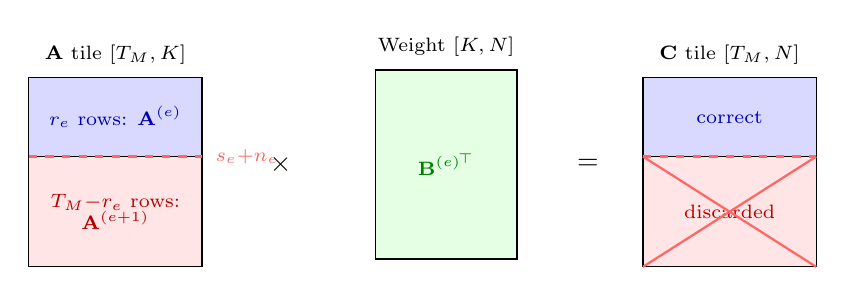
\begin{tikzpicture}[
  box/.style={draw, minimum width=2.2cm, inner sep=0pt, outer sep=0pt},
  valid/.style={box, fill=blue!15, minimum height=#1},
  garbage/.style={box, fill=red!10, minimum height=#1},
  label/.style={font=\scriptsize},
  arr/.style={-{Stealth[length=4pt]}, thick},
]
% --- A tile ---
\node[valid=1.0cm] (av) at (0, 0.8) {};
\node[label, text=blue!70!black] at (av) {$r_e$ rows: $\mathbf{A}^{(e)}$};
\node[garbage=1.4cm] (ag) at (0, -0.4) {};
\node[label, text=red!70!black, align=center] at (ag) {$T_M{-}r_e$ rows:\\$\mathbf{A}^{(e+1)}$};
\node[label, anchor=south] at (0, 1.35) {$\mathbf{A}$ tile $[T_M, K]$};
% dashed boundary
\draw[dashed, thick, red!60] (-1.1, 0.3) -- (1.1, 0.3);
\node[label, anchor=west, text=red!60] at (1.15, 0.3) {$s_e{+}n_e$};

% --- B matrix ---
\node[box, fill=green!10, minimum height=2.4cm, minimum width=1.8cm]
  (B) at (4.2, 0.2) {};
\node[label, text=green!50!black] at (B) {${\mathbf{B}^{(e)}}^{\!\top}$};
\node[label, anchor=south] at (4.2, 1.45) {Weight $[K, N]$};

% --- multiply arrow ---
\node[font=\normalsize] at (2.1, 0.2) {$\times$};

% --- equals ---
\node[font=\normalsize] at (6.0, 0.2) {$=$};

% --- C tile ---
\node[valid=1.0cm] (cv) at (7.8, 0.8) {};
\node[label, text=blue!70!black] at (cv) {correct};
\node[garbage=1.4cm] (cg) at (7.8, -0.4) {};
\node[label, text=red!70!black] at (cg) {discarded};
\node[label, anchor=south] at (7.8, 1.35) {$\mathbf{C}$ tile $[T_M, N]$};
\draw[dashed, thick, red!60] (6.7, 0.3) -- (8.9, 0.3);

% --- strike-through for discarded ---
\draw[thick, red!60] (6.7, -1.1) -- (8.9, 0.3);
\draw[thick, red!60] (6.7, 0.3) -- (8.9, -1.1);
\end{tikzpicture}
\caption{Last tile of an interior expert ($e < E$). The TMA load
reads $r_e$ valid rows from expert~$e$ and $T_M - r_e$ rows from
expert~$e{+}1$. MMA computes all $T_M$ output rows, but only the
first $r_e$ rows are written back; the remaining rows (crossed out)
are discarded by the predicated store.}
\label{fig:partial-tile}
\end{figure}

For the last expert ($e = E$), the overflow rows have indices
$\geq S$, which fall outside the allocated region of~$\mathbf{A}$
and would cause an out-of-bounds memory access.
RapidsGEMM handles this by enabling the TMA out-of-bounds fill
mode~\cite{nvidia_cuda_programming_guide}: when TMA encounters a
coordinate $\geq$ \texttt{globalDim}, it zero-fills the corresponding
shared-memory elements. The output tile becomes
\begin{equation}
  \mathbf{C}_{\text{tile}} =
    \mathbf{A}[\underbrace{s_E{+}tT_M : s_E{+}tT_M{+}r_E}_{
      \text{expert } E}\;|\;
    \underbrace{0, \dots, 0}_{
      T_M{-}r_E \text{ zero-filled rows}},\; :]\;
    {\mathbf{B}^{(E)}}^{\!\top}.
\label{eq:tile-matmul-last}
\end{equation}
The zero-filled rows contribute nothing to the MMA result, so the load
is safe without additional memory allocation. This is a descriptor
flag set once at launch time; no per-tile conditional logic is needed.

\paragraph{Padding-free stores.}
The store path is the same for interior experts and the last expert.
Let the tile starting at row~$m$ for expert~$e$ have
$a = \min(s_e + n_e - m,\; T_M)$ valid rows (clamped to $T_M$ for
full tiles). Two write-back paths are used:
\begin{itemize}
  \item \textbf{Bulk store} ($a = T_M$): the tile falls
    within expert~$e$'s region. The kernel writes the full
    $T_M \times N$ result tile through a single TMA store.
  \item \textbf{Predicated store} ($a < T_M$): the tile is the last
    (partial) tile of expert~$e$. The kernel casts the accumulator to
    the output type in registers and issues per-element predicated
    stores, writing only the $a$~valid rows and discarding the
    remaining $T_M - a$ rows.
\end{itemize}
Regardless of whether the overflow rows came from the next
expert's data (interior expert) or from TMA zero-fill (last expert),
the same predicated store logic discards them. At most one tile per
expert uses the predicated store: for $E$~experts
tiling a total of $\sum_{e} \lceil n_e / T_M \rceil$ tiles, at most
$E$ tiles (one per expert) use predicated stores while all others use
bulk stores.

%---------------------------------------------------------------------
\subsection{Padding-Free K-GEMM}
%---------------------------------------------------------------------

\paragraph{Why the M-GEMM approach fails for K-GEMM.}
In M-GEMM the token dimension~$n_e$ is the output row dimension.
When a tile overflows into the next expert's rows, the foreign rows
produce extra output rows that can be discarded by a predicated store
(\S\ref{sec:gemm-inventory}).
In K-GEMM, however, the token dimension~$n_e$ is the \emph{reduction}
dimension.
The kernel tiles the reduction axis with a fixed tile size~$T_K$ and
accumulates partial sums across $\lceil n_e / T_K \rceil$ tiles per
expert.
When the last reduction tile of expert~$e$ extends beyond $n_e$,
the overflow rows are not written to separate output locations --- they
are accumulated into the \emph{same} output elements as the valid rows.

To see why this is fatal, consider the last reduction tile for an
interior expert ($e < E$).
Let $r_e = n_e \bmod T_K$ be the number of valid rows in this tile.
The TMA load reads $r_e$ rows from expert~$e$ and $T_K - r_e$
rows from expert~$e{+}1$.
Both operands $\mathbf{A}$ and $\mathbf{B}$ load from the same
row interval, so the accumulated partial sum becomes
\begin{equation}
  \mathbf{C}_{\text{tile}} =
    \underbrace{{\mathbf{A}^{(e)}_{\text{tail}}}^{\!\top}
               \,\mathbf{B}^{(e)}_{\text{tail}}}_{\text{correct}}
    \;+\;
    \underbrace{{\mathbf{A}^{(e+1)}_{\text{head}}}^{\!\top}
               \,\mathbf{B}^{(e+1)}_{\text{head}}}_{\text{error}},
\label{eq:kgemm-contamination}
\end{equation}
where the subscripts ``tail'' and ``head'' denote the $r_e$ valid and
$T_K - r_e$ foreign rows, respectively.
The error term is generally non-zero and is added directly to the
accumulator.
Because a single output element receives contributions from every
reduction tile, there is no way to remove the error term after the
fact --- neither predicated stores nor output masking can undo an
incorrect partial sum.
Therefore the M-GEMM strategy of ``load freely, write selectively''
does not apply to K-GEMM.

\paragraph{Key idea: per-expert TMA descriptors with zero-fill.}
Instead of tolerating overflow and filtering the output, RapidsGEMM
prevents overflow at the input.
The idea is to give each expert its own TMA descriptor whose
\texttt{globalDim} along the reduction axis equals the expert's true
token count~$n_e$.
When TMA loads a reduction tile that extends beyond~$n_e$, the
out-of-bounds positions are zero-filled automatically.
Because a zero-valued row contributes nothing to the matrix product,
the partial sum from the last tile equals the partial sum over only the
$r_e$ valid rows.
This eliminates the error term in Eq.~\eqref{eq:kgemm-contamination}
without padding the global memory buffer.

\paragraph{On-device descriptor modification.}
A standard TMA descriptor is created on the host before kernel launch.
Creating $E$ separate descriptors on the host and passing all of them
as kernel arguments is impractical when $E$ is large or when the token
counts are determined at runtime.
CUDA addresses this problem with on-device modification of tensor map
descriptors, available on \texttt{sm\_90a} and later
architectures~\cite{nvidia_cuda_programming_guide,nvidia_ptx_isa}.
The PTX instruction set provides \texttt{tensormap.replace}, which can
overwrite individual fields of a 128-byte tensor map descriptor stored
in shared memory~\cite{nvidia_ptx_isa}.
Fields such as the base address (\texttt{globalAddress}), tensor
dimensions (\texttt{globalDim}), and inter-row strides
(\texttt{globalStrides}) can each be replaced independently while the
remaining fields retain their original
values~\cite{nvidia_cuda_programming_guide}.
After modification, the updated descriptor must be copied from shared
memory to a global memory location and made visible to the TMA hardware
through a release--acquire fence
pair~\cite{nvidia_cuda_programming_guide}.

RapidsGEMM uses this mechanism as follows.
Before launch, the host creates a single \emph{template} descriptor via
\texttt{cuTensorMapEncodeTiled}~\cite{nvidia_cuda_toolkit} with
placeholder values for the base address and tensor dimensions; all
other fields (tile size, swizzle pattern, out-of-bounds fill mode,
etc.)\ are set to their final values.
Inside the kernel, each CTA processes tiles from one expert at a time.
When a CTA transitions to a new expert~$e$, one elected thread
performs three steps:
\begin{enumerate}
  \item Copy the template descriptor from kernel parameters into
    shared memory.
  \item Overwrite the base address with expert~$e$'s data pointer and
    the reduction-axis dimension with~$n_e$, using
    \texttt{tensormap.replace}~\cite{nvidia_ptx_isa}.
  \item Copy the modified descriptor from shared memory to a global
    memory slot and issue a release fence so that the TMA hardware can
    read the updated
    descriptor~\cite{nvidia_cuda_programming_guide}.
\end{enumerate}
Before the next TMA load, the CTA executes an acquire fence on the
global descriptor~\cite{nvidia_cuda_programming_guide}.
All subsequent TMA loads for expert~$e$ then reference this updated
descriptor, and any coordinate that exceeds~$n_e$ along the reduction
axis is zero-filled.

\paragraph{Correctness.}
For each expert~$e$, the K-GEMM accumulates over
$\lceil n_e / T_K \rceil$ reduction tiles.
Every full tile ($t < \lceil n_e / T_K \rceil - 1$) lies entirely
within expert~$e$'s data and contributes an exact partial sum.
The last tile loads $r_e = n_e \bmod T_K$ valid rows and
$T_K - r_e$ zero-filled rows.
Because each zero-filled row contributes a zero outer product, the
partial sum from this tile equals
\begin{equation}
  \mathbf{C}_{\text{tile}} =
    {\mathbf{A}^{(e)}_{\text{tail}}}^{\!\top}
    \,\mathbf{B}^{(e)}_{\text{tail}}
    \;+\;
    \underbrace{\mathbf{0}^{\!\top}\,\mathbf{0}}_{=\,\mathbf{0}}.
\label{eq:kgemm-zerofill}
\end{equation}
Summing over all tiles yields
$\mathbf{C}^{(e)} = {\mathbf{A}^{(e)}}^{\!\top}\,\mathbf{B}^{(e)}$,
identical to the result of the unpadded computation.
The descriptor update adds a small overhead per expert transition, but
this cost is amortised over the $\lceil n_e / T_K \rceil$ tiles
processed for each expert.

%=============================================================================
\section{Experiments}
\label{sec:experiments}
%=============================================================================

We evaluate RapidsGEMM at three levels of granularity: (1)~grouped GEMM
kernel microbenchmarks, (2)~single MoE layer forward--backward pass, and
(3)~end-to-end MoE training throughput with expert parallelism.
All experiments compare our padding-free grouped GEMM against the
padded baseline under two precisions: BF16 and MXFP8.
We target NVIDIA Blackwell (B200) GPUs as the primary platform.

%---------------------------------------------------------------------
\subsection{Experimental Setup}
\label{sec:exp-setup}
%---------------------------------------------------------------------

\paragraph{Hardware.}
All experiments run on a single node with eight NVIDIA B200 (SM100a) GPUs
connected via NVLink.

\paragraph{Software stack.}
We implement RapidsGEMM as a drop-in replacement for the grouped GEMM
kernel in two open-source MoE training frameworks:
\begin{itemize}
  \item \textbf{TorchTitan + TorchAO}~\cite{torchtitan2025,torchao2025}:
    TorchAO provides the \texttt{torch.\_scaled\_grouped\_mm} interface
    for MXFP8 grouped GEMMs.
    We replace the underlying CUTLASS grouped GEMM kernel with RapidsGEMM
    and keep the quantization and scale-rearrangement path unchanged.
    We also port BF16 grouped GEMM via
    \texttt{torch.\_grouped\_mm}.
  \item \textbf{Megatron-Core}~\cite{nvidia2026megatronmoe}:
    Megatron-Core's \texttt{TEGroupedMLP} dispatches to either
    multi-stream cuBLASLt GEMMs or CUTLASS grouped GEMMs.
    We add a RapidsGEMM backend that reads the device-side
    tokens-per-expert tensor and calls our padding-free kernel
    directly, avoiding the fused-padding permutation kernel.
\end{itemize}
For both frameworks, the integration amounts to replacing the
grouped GEMM call site (and removing the upstream padding logic)
while keeping all other components --- routing, permutation,
quantization, communication, and compilation --- identical between
the baseline and RapidsGEMM runs.

\paragraph{Model shapes.}
We benchmark on two representative MoE architectures:
\begin{itemize}
  \item \textbf{Llama4-Scout-like}~\cite{llama4scout2025}:
    $D = 5120$, $F = 8192$, $E_{\text{total}} = 16$,
    top-$k = 1$, sequence length $= 8192$.
  \item \textbf{DeepSeek-V3-like}~\cite{deepseekv3}:
    $D = 7168$, $F = 2048$, $E_{\text{total}} = 256$,
    top-$k = 8$, sequence length $= 4096$.
\end{itemize}
These two models span a wide range of expert granularity:
Llama4-Scout has few, large experts while DeepSeek-V3 has many,
small experts --- the latter being the harder case for grouped GEMM
because per-expert token counts are smaller and more irregular.

\paragraph{Precision configurations.}
Each benchmark is run under two precisions:
(a)~BF16, using \texttt{torch.\_grouped\_mm}, and
(b)~MXFP8 (E4M3 elements, E8M0 32-block scales), using
\texttt{torch.\_scaled\_grouped\_mm}.
For MXFP8, we report the total time including dynamic quantization
and scale-factor rearrangement, since these overheads are part of
the end-to-end cost.

\paragraph{Token distribution.}
To stress-test padding overhead, we evaluate under three token
distributions per expert:
(i)~\emph{uniform}: all experts receive the same number of tokens
(best case for padding, since $n_e$ is likely a multiple of the tile
size);
(ii)~\emph{skewed}: token counts follow a Zipf distribution
($\alpha = 1.1$), mimicking realistic load imbalance;
(iii)~\emph{forced-balanced}: the router enforces equal token counts
(used in end-to-end training benchmarks following
Megatron-Core's practice~\cite{nvidia2026megatronmoe}).

\paragraph{Metrics.}
We report:
\emph{latency} (microseconds) for kernel-level benchmarks,
\emph{tokens per second} (tokens/s) for MoE layer and end-to-end
benchmarks, and
\emph{TFLOPS per GPU} for end-to-end benchmarks.
Speedup is computed as
$\text{speedup} = t_{\text{baseline}} / t_{\text{RapidsGEMM}}$
where the baseline uses padded grouped GEMM.

%---------------------------------------------------------------------
\subsection{Experiment~1: Grouped GEMM Kernel Microbenchmarks}
\label{sec:exp-kernel}
%---------------------------------------------------------------------

\paragraph{Goal.}
Isolate the performance gain of padding-free grouped GEMM at the
kernel level, independent of quantization, routing, or communication.

\paragraph{Design.}
We benchmark the six grouped GEMMs listed in
Table~\ref{tab:gemm-inventory} (four M-GEMMs and two K-GEMMs)
individually.
For each GEMM, we fix the model dimensions ($D$, $F$, $E$) and
vary the total token count $S$ across
$\{8192, 16384, 32768, 65536, 131072\}$.
At each $S$, we test both the uniform and skewed token distributions.
Each configuration is run under both BF16 and MXFP8.

\paragraph{Baseline.}
The baseline pads each expert's token count to the next multiple
of 128 (following DeepGEMM's convention~\cite{deepgemm2025})
before calling the grouped GEMM kernel.

\paragraph{Expected figures.}
\begin{itemize}
  \item \textbf{Figure~A} (2 subfigures: Llama4, DeepSeek-V3):
    Bar chart of kernel latency for the six GEMMs.
    $x$-axis: GEMM index (1--6); bars grouped by
    \{baseline-BF16, RapidsGEMM-BF16, baseline-MXFP8,
    RapidsGEMM-MXFP8\}.
    Fixed $S = 131072$, skewed distribution.
    Shows per-GEMM speedup.
  \item \textbf{Figure~B} (2 subfigures: M-GEMM, K-GEMM):
    Line plot of speedup vs.\ total token count~$S$.
    $x$-axis: $S$; $y$-axis: speedup.
    Lines for \{BF16-uniform, BF16-skewed, MXFP8-uniform,
    MXFP8-skewed\}.
    Shows how speedup scales with problem size and imbalance.
  \item \textbf{Table}: Breakdown of time saved from removed padding
    (memory bandwidth) vs.\ removed computation on padded zeros.
\end{itemize}

\paragraph{Resources.}
Single B200 GPU; each configuration takes $\sim$5 seconds;
total: $\sim$2 hours including warm-up.

%---------------------------------------------------------------------
\subsection{Experiment~2: Single MoE Layer Forward--Backward}
\label{sec:exp-layer}
%---------------------------------------------------------------------

\paragraph{Goal.}
Measure the end-to-end speedup of RapidsGEMM for the full MoE layer
computation, including routing, permutation, all six grouped GEMMs
(forward + backward), activation functions, and quantization
(for MXFP8).

\paragraph{Design.}
We benchmark a single MoE layer's forward + backward pass.
Following the TorchAO benchmark
protocol~\cite{torchao2025}, we fix $E$ experts on a single GPU
(simulating EP=$E$) and vary the local batch size to control the
total token count.
We test:
\begin{itemize}
  \item Llama4-Scout shapes: $S = 131072$, $E_{\text{local}} = \{1, 2, 4, 8, 16\}$.
  \item DeepSeek-V3 shapes: $S = 131072$, $E_{\text{local}} = \{1, 2, 4, 8\}$.
\end{itemize}
Varying $E_{\text{local}}$ is important: with more local experts,
each expert receives fewer tokens on average, making per-expert
token counts smaller and less aligned --- this amplifies padding waste.

\paragraph{Baseline.}
The TorchAO / Megatron-Core default path with padded grouped GEMM.

\paragraph{Expected figures.}
\begin{itemize}
  \item \textbf{Figure~C} (2 subfigures: Llama4, DeepSeek-V3):
    Grouped bar chart.
    $x$-axis: $E_{\text{local}}$; bars: \{baseline-BF16,
    RapidsGEMM-BF16, baseline-MXFP8, RapidsGEMM-MXFP8\};
    $y$-axis: layer forward+backward time (ms).
    Annotate speedup above each RapidsGEMM bar.
  \item \textbf{Figure~D}:
    Stacked bar chart showing time breakdown by component
    (routing + permute, grouped GEMM fwd, grouped GEMM bwd,
    quantization, other) for baseline vs.\ RapidsGEMM under MXFP8.
    Shows where the savings come from.
\end{itemize}

\paragraph{Resources.}
Single B200 GPU; each configuration takes $\sim$10 seconds with
200 warm-up + 100 timed iterations; total: $\sim$1 hour.

%---------------------------------------------------------------------
\subsection{Experiment~3: End-to-End MoE Training Throughput}
\label{sec:exp-e2e}
%---------------------------------------------------------------------

\paragraph{Goal.}
Demonstrate that the kernel-level speedup translates to end-to-end
training throughput improvements in a realistic distributed setting,
where communication, memory management, and compilation interact with
the grouped GEMM.

\paragraph{Design.}
We run end-to-end training (200 steps, measuring median tokens/s)
on Llama4-Scout and DeepSeek-V3-like models at multiple scales:

\begin{table}[h]
\centering
\small
\caption{End-to-end benchmark configurations (single node, 8$\times$ B200).}
\label{tab:e2e-configs}
\begin{tabular}{@{}llcccc@{}}
\toprule
Model & GPUs & EP & FSDP & TP \\
\midrule
Llama4-Scout & 4 & 4 & 4 & 1 \\
Llama4-Scout & 8 & 8 & 8 & 1 \\
\midrule
DeepSeek-V3 & 4 & 4 & 4 & 1 \\
DeepSeek-V3 & 8 & 8 & 8 & 1 \\
\bottomrule
\end{tabular}
\end{table}

For each configuration, we compare four settings:
(a)~padded BF16,
(b)~RapidsGEMM BF16,
(c)~padded MXFP8,
(d)~RapidsGEMM MXFP8.
All runs use \texttt{torch.compile}, FSDP2, and the same
activation checkpointing mode.

\paragraph{Integration in TorchTitan.}
We port RapidsGEMM into TorchTitan by:
\begin{enumerate}
  \item Registering a new grouped GEMM backend in TorchAO's
    \texttt{moe\_training} module that calls RapidsGEMM instead of
    the default CUTLASS kernel.
  \item Modifying the MoE layer's token permutation path to
    skip padding when RapidsGEMM is selected, since our kernel
    handles unaligned token counts natively.
  \item Keeping the \texttt{MXGroupedMMConverter} and
    \texttt{MXLinearConverter} configuration identical to the
    baseline, so the only variable is the grouped GEMM kernel.
\end{enumerate}

\paragraph{Integration in Megatron-Core.}
We add a RapidsGEMM backend to the \texttt{TEGroupedMLP} module:
\begin{enumerate}
  \item Replace the multi-stream cuBLASLt / CUTLASS grouped GEMM
    call with RapidsGEMM, passing the device-side
    \texttt{tokens\_per\_expert} tensor directly.
  \item Disable the fused-padding permutation kernel
    (Section~5.4.1 of~\cite{nvidia2026megatronmoe}), since
    RapidsGEMM eliminates the alignment requirement on
    per-expert token counts.
  \item Verify CUDA Graph compatibility, since RapidsGEMM
    reads token counts from device memory and does not require
    host--device synchronization.
\end{enumerate}

\paragraph{Expected figures.}
\begin{itemize}
  \item \textbf{Figure~E}:
    Grouped bar chart of training throughput (tokens/s/GPU).
    $x$-axis: GPU count (4, 8); bars: \{padded-BF16,
    RapidsGEMM-BF16, padded-MXFP8, RapidsGEMM-MXFP8\}.
    One subfigure per model.
    Annotate speedup over the padded baseline.
  \item \textbf{Figure~F}:
    TFLOPS/GPU comparison at 8-GPU scale for both models.
    Shows how RapidsGEMM narrows the gap to peak hardware throughput.
  \item \textbf{Table}: Peak memory (GB) for each configuration,
    verifying that RapidsGEMM does not increase memory usage
    (and may reduce it by eliminating padded buffers).
\end{itemize}

\paragraph{Resources.}
All runs use a single node with 8~B200 GPUs.
Each configuration takes $\sim$30 minutes (200 training steps).
With 4~configurations $\times$ 4~model-GPU combinations $= 16$ runs,
the total is $8 \times 0.5\text{h} \times 16 = 64$ GPU-hours.

%---------------------------------------------------------------------
\subsection{Experiment~4: Ablation Studies}
\label{sec:exp-ablation}
%---------------------------------------------------------------------

We conduct two ablation studies to isolate the contributions of
individual components.

\paragraph{Ablation A: M-GEMM only vs.\ K-GEMM only vs.\ both.}
Using the single MoE layer benchmark (Experiment~2), we enable
padding-free M-GEMM alone, padding-free K-GEMM alone, and both
together.
This separates the contribution of each technique.
We expect K-GEMM to contribute a larger share of the speedup in the
backward pass (where two of the four GEMMs are K-GEMMs), while
M-GEMM dominates in the forward pass.

\paragraph{Ablation B: Impact of token imbalance.}
Using the kernel microbenchmark (Experiment~1), we sweep the Zipf
parameter $\alpha \in \{0, 0.5, 1.0, 1.5, 2.0\}$ (where
$\alpha = 0$ is uniform).
Higher $\alpha$ creates more skew, meaning some experts receive
very few tokens.
Experts with small $n_e$ suffer the most padding waste, so we expect
RapidsGEMM's speedup to increase with $\alpha$.

\paragraph{Expected figures.}
\begin{itemize}
  \item \textbf{Figure~G}: Stacked bar chart showing layer time
    with M-GEMM only, K-GEMM only, and both enabled.
  \item \textbf{Figure~H}: Line plot of kernel speedup vs.\ Zipf
    $\alpha$ for M-GEMM and K-GEMM separately.
\end{itemize}

%---------------------------------------------------------------------
\subsection{Choice of Benchmark Models}
\label{sec:exp-model-choice}
%---------------------------------------------------------------------

We select Llama4-Scout and DeepSeek-V3 for two reasons:
they cover opposite ends of the MoE design spectrum, and they are
the most widely benchmarked MoE architectures in the open-source
ecosystem, making our results directly comparable to existing
baselines.

\paragraph{Complementary stress tests.}
Llama4-Scout has 16 experts with top-1 routing.
Each expert receives many tokens on average ($S / 16$), so
per-expert token counts are relatively large and more likely to be
tile-aligned.
This is the easy case for padding: padding waste is a small fraction
of each expert's work.
If RapidsGEMM still shows speedup here, the benefit is not limited
to pathological cases.
DeepSeek-V3 has 256 experts with top-8 routing.
Each expert receives far fewer tokens, and per-expert token counts
are small and irregular --- some experts may get only tens of tokens.
This is the hard case for padding: rounding each expert's token
count up to 128 wastes a large fraction of the GEMM work.
This is where RapidsGEMM's advantage should be most visible.

\paragraph{Comparability with prior work.}
Both models appear in the benchmarks of every reference framework
we target.
TorchAO~\cite{torchao2025} reports autograd-function and
single-layer benchmarks on both Llama4-Scout shapes
($K{=}5120$, $N{=}8192$) and DeepSeek-V3 shapes
($K{=}7168$, $N{=}2048$).
TorchTitan~\cite{torchtitan2025} reports end-to-end MoE training
throughput on Llama4-Scout at 512-GPU scale.
Megatron-Core~\cite{nvidia2026megatronmoe} uses DeepSeek-V3 as its
primary case study and reports up to 1048~TFLOPS/GPU on GB200.
Using the same shapes lets reviewers compare our results against
these published baselines directly.

%=============================================================================
\section{Conclusion}
%=============================================================================

%=============================================================================
% References (manually maintained)
%=============================================================================
\begin{thebibliography}{9}

\bibitem{shazeer2017outrageously}
N.~Shazeer, A.~Mirhoseini, K.~Maziarz, A.~Davis, Q.~Le, G.~Hinton, and J.~Dean,
``Outrageously large neural networks: The sparsely-gated mixture-of-experts layer,''
\emph{arXiv preprint arXiv:1701.06538}, 2017.

\bibitem{gale2023megablocks}
T.~Gale, D.~Narayanan, C.~Young, and M.~Zaharia,
``{MegaBlocks}: Efficient sparse training with mixture-of-experts,''
\emph{Proceedings of Machine Learning and Systems}, vol.~5, 2023.

\bibitem{nvidia2026megatronmoe}
NVIDIA,
``Scalable training of mixture-of-experts models with {Megatron Core},''
\emph{arXiv preprint arXiv:2603.07685}, 2026.

\bibitem{tmaadaptive2025}
Y.~Yang, J.~Li, and others,
``{TMA-Adaptive Grouped GEMM}: Padding-free {TMA} access for irregular
grouped {GEMM} on {GPU},''
\emph{arXiv preprint}, 2025.

\bibitem{deepgemm2025}
C.~Zhao, L.~Zhao, J.~Li, and Z.~Xu,
``{DeepGEMM}: Clean and efficient {FP8} {GEMM} kernels with fine-grained
scaling,''
\url{https://github.com/deepseek-ai/DeepGEMM}, 2025.

\bibitem{nvidia_cuda_programming_guide}
NVIDIA,
``{CUDA Programming Guide},''
\url{https://docs.nvidia.com/cuda/cuda-programming-guide/}, 2025.

\bibitem{nvidia_cuda_toolkit}
NVIDIA,
``{CUDA Toolkit Documentation: cuTensorMapEncodeTiled},''
\url{https://docs.nvidia.com/cuda/cuda-driver-api/}, 2025.

\bibitem{nvidia_ptx_isa}
NVIDIA,
``{PTX ISA Reference},''
\url{https://docs.nvidia.com/cuda/parallel-thread-execution/}, 2025.

\bibitem{torchtitan2025}
PyTorch Team,
``{TorchTitan}: A native {PyTorch} large model training framework,''
\url{https://github.com/pytorch/torchtitan}, 2025.

\bibitem{torchao2025}
PyTorch Team,
``{TorchAO}: {PyTorch} architecture optimization library,''
\url{https://github.com/pytorch/ao}, 2025.

\bibitem{llama4scout2025}
Meta AI,
``{Llama 4}: The {Llama} herd is getting bigger,''
\url{https://ai.meta.com/blog/llama-4-multimodal-intelligence/}, 2025.

\bibitem{deepseekv3}
DeepSeek-AI,
``{DeepSeek-V3} technical report,''
\emph{arXiv preprint arXiv:2412.19437}, 2024.

\end{thebibliography}

\end{document}